\newcommand{\Swift}{SWIFT-pidt}


\chapter{\Peano's particle support and \Swift}
\label{section:pidt}


% \begin{figure}[htb]
 \begin{center}
  
\includegraphics[width=0.2\textwidth]{61_pidt/ExCALIBUR.png}
 \end{center}


\noindent
\Swift\ is a SWIFT (SPH With Inter-dependent Fine-grained
Tasking) clone which combines the SWIFT SPH kernels
(tasks) with Peano's particle-in-dual-tree concept.
The original SWIFT codes is available from \url{https://swift.dur.ac.uk}.
\Peano's particle handling is a follow-up to the 2015 paper ``Two Particle-in-Grid Realisations on Spacetrees'' (\url{https://arxiv.org/abs/1508.02435}).
The integration of the SWIFT kernels and \Peano\ has been made possible by the
EPSRC ExCALIBUR grants Massively Parallel Particle Hydrodynamics
for Engineering and Astrophysics (EP/V001523/1) and PAX-SPH.
\Swift\ is realised as Python layer on top of \Peano\ and brings \Peano's core, 
its particle toolsbox and SWIFT together.
You can still use solely \Peano\ and its particles without SWIFT if you prefer
to work more low-level or without SPH\footnote{\ExaHyPE's tracer realisation
goes internally down this route.}.





\begin{framed}
\paragraph*{A first \Peano\ pidt run (native usage of particle interface)}
\begin{itemize}
  \item Configure \Peano\ with the flags \texttt{--enable-particles}:
  \begin{code}
libtoolize; aclocal; autoconf; autoheader; cp src/config.h.in .; automake --add-missing
./configure --enable-particles
  \end{code}
   These are the two mandatory extensions. You might want to add further options.
  \item Recompile your \Peano\ code. This should give you a couple of
  \texttt{ToolboxParticles} libraries in the \texttt{src/toolbox/particles}
  subdirectory.
  \item Ensure that \texttt{python} subdirectory is in your Python search path
  and
  \item run the Jupyter notebook in \texttt{examples/particles/sph}: 
  \begin{code}
export PYTHONPATH=../../../python/
jupyter-notebook peano-sph.ipynb
  \end{code}
%   \noindent
%   or---if you don't like Jupyter notebooks---type in
%   \begin{code}
% export PYTHONPATH=../../../python/
% ipython3 example-scripts/finitevolumes-with-ExaHyPE2-benchmark.py --h 0.1
% ./peano4
%   \end{code}
\end{itemize}
\end{framed}


\section{\Swift}

Our interface for \Swift\ is almost complete realised in Python.
Only specialised potentials have to be injected via C++.


\subsection{Set up the simulator}


\subsection{Introduce a new particle}

The generation of a particle is straightforward. We employ a tool called
DaStGen2 which really just is a set of Python classes which represent the 
attributes of a C++ class. We build up a set of Python objects and \Swift\
eventually dumps them into C++ code from which it is embedded into the 
actual simulator.   

\begin{code}
import dastgen2

particle = peano4.toolbox.particles.Particle("Particle")

v_attr = peano4.dastgen2.Peano4DoubleArray("v","Dimensions")
mass_attr = dastgen2.attributes.Double("mass")

particle.data.add_attribute(v_attr)
particle.data.add_attribute(mass_attr)


@todo something fancy in here that adds a new species
\end{code}

\begin{remark}
 Though conceptionally a plain C++ pretty printer, the DaStGen2 Python API
 can create some fancy C++ annotations. You can, for example, specify ranges
 in which integers live, or you can prescribe the precision you wanna have 
 for floating point values. If you have a specialised LLVM compiler, these
 annotations will be used to generate aggressively optimised code.
\end{remark}



\subsection{IO control}

\Peano\ dumps a lot of information to the terminal by default. Consult
Section~\ref{section:logging:log-filter} for some remarks on how to filter the
output properly.


% \subsection{todo}
% Python API muss
% \begin{itemize}
%   \item swift2.filter-file erzeugen und lesen
%   \item Load balancing offerieren
% \end{itemize}


\subsection{High-performance computing}
\label{section:particles:swift:hpc}

To use \Peano's high-performance computing features, you have to configure your
baseline code properly.
That is, you need to invoke \texttt{./configure} with an appropriate
\texttt{--with-multithreading=...} call to enable multithreading, 
you need to invoke it with \texttt{--with-mpi=...} for MPI support, and you need
to specify \texttt{--enable-gpus=...} if you want to use accelerators.
Furthermore, you will have to enable \Peano's load balancing toolbox
(\texttt{--enable-loadbalancing}), unless you want to implement load balancing all on
your own.



\section{Native \Peano\ with particles}

\Peano's particle code is lightweight.
There are some C++ building blocks, but the majority of its features are
available through the Python API as
\texttt{toolbox.particles}.
You will need

\begin{code}
import peano4.toolbox.particles
\end{code}

\noindent
I assume that you are familiar from hereon with \Peano's basics, i.e.~you know 
how to create a project, 

\subsection{Introduce a new particle}

With the Python API, the generation of a particle is straightforward:

\begin{code}
import dastgen2


particle = peano4.toolbox.particles.Particle("Particle")

v_attr = peano4.dastgen2.Peano4DoubleArray("v","Dimensions")
mass_attr = dastgen2.attributes.Double("mass")

particle.data.add_attribute(v_attr)
particle.data.add_attribute(mass_attr)

particles = peano4.toolbox.particles.ParticleSet(particle)
\end{code}

\begin{remark}
 Though conceptionally a plain C++ pretty printer, the DaStGen2 Python API
 can create some fancy C++ annotations. You can, for example, specify ranges
 in which integers live, or you can prescribe the precision you wanna have 
 for floating point values. If you have a specialised LLVM compiler, these
 annotations will be used to generate aggressively optimised code.
\end{remark}


\noindent
The \Peano\ particle has some additional attributes as they are discussed in 
Section \ref{section:swift:backbone:data-model} and thereafter. 
For the user, it is usually sufficient to recognise that each particle by 
default has a position \texttt{x} and and a cut-off radius
\texttt{cutOffRadius}.
You can query and modify both values through \texttt{setX}, \texttt{getX},
\texttt{getCutOffRadius} and \texttt{setCutOffRadius}, respectively.


We next add the particles to the project and we notify the vertices that there 
are particles which have to be administered. 
I discuss why and how pidt uses vertices in Section
\ref{section:swift:backbone:dual-trees} though users might (initially) skip such
background info. 

\begin{code}
project.datamodel.add_global_object(particle)
project.datamodel.add_vertex(particles)
\end{code}

\noindent
Once you have added the particle and the particle container \texttt{particles}
to your \Peano\ datamodel, you have to inform all solver steps that they have to
administer the particles.

\begin{code}
create_grid.use_vertex(particles)
\end{code}

\noindent
Let's assume that our project is spanning the namespace
\texttt{examples::someparticles}.
 In the example above where our particle is
called \texttt{Particle}, we will end up with two classes:
\linebreak
\texttt{examples::someparticles::globaldata::Particle} is the actual particle
class. 
When you open the generated C++ code, you'll recognise that it is a 1:1 mapping
of the Python attributes onto a C++ class with some additional routines used by
\Peano\ internally.
There is a further class
\texttt{examples::someparticles::vertexdata::ParticleSet}.
As the name says, this is the actual data associated with each vertex.
It is a specialisation of \texttt{std::vector} over pointers to
\texttt{examples::someparticles::globaldata::Particle}.

We summarise that each vertex holds a vector to pointers over particles.
The actual particles reside on the heap.



\subsection{Create particles}

To create a particle, you in principle just allocate it on the heap, and then
you add it to its nearest vertex.
Furthermore, there are some mandatory attributes that aways have to be set. 
Therefore, I recommend that you use the toolbox' initialisation routine to set
up particles correctly.


In principle, it does not matter where you create the particle.
You can do so in \texttt{touchCellFirstTime()} or in a cell event. 
I usually use a cell event:


\begin{code}
#include "toolbox/particles/ParticleFactory.h"

examples::someparticles::globaldata::Particle* myNewParticle = 
  new examples::someparticles::globaldata::Particle();
  
// assume x and cutOffRadius are set to something meaningful
toolbox::particles::init( *myNewParticle, x, cutOffRadius );

toolbox::particles::init( *myNewParticle, x, cutOffRadius );

\end{code}


\subsection{Move particles}

\begin{definition}
 In \Swift's \emph{dual tree} storage scheme, particles are always stored to
 their nearest neighbour.
\end{definition}


To create a particle, you in principle just allocate it on the heap, and then
you add it to its nearest vertex.


\begin{definition}
 In \Swift's \emph{dual tree} storage scheme, we always hold the
 complete spacetree with all tree (grid) levels. Particles are always stored on
 the finest mesh (tree) level where the mesh size is bigger than the particle's
 cut-off radius. 
 Different particles with different cut-off radii might thus be stored on
 different tree levels.
\end{definition}


\subsection{Particle-particle interaction}




Per cell, the code assembles a \texttt{local set}. 
This is a list of pointers to those particles that are associated to a cell's
$2^d$ vertices.
With the local set, you can make particles held on one resolution level
interact with each other.
You get an cubic area of $2h$ side-lenght per cell:
As a particle is always associated to its closest vertex, the local set holds all particles whose cut-off radius overlap with the cell. 


Adaptivity and particles with different cut-off are not yet captured through the
local set notion.
There's thus a second set that I call active set. 
The active set is the local set plus all local sets that have been active on
coarser levels within the tree.

\begin{definition}
 The active set is built up top-down while we run through the
 tree.
 So it is a data structure that grows and shrinks while you run through the
 meshes.
 The local set \texttt{localParticles} is created on-the-fly every time you hit
 a cell or a vertex.
 Do not alter the active set: You can modify the values of the particles within
 an active set, but you should not add or remove entries from it.
 The local set can be modified.
\end{definition}


If you use the \texttt{toolbox.particles.ParticleParticleInteraction} action
set, you pass it some C source code that works with the particles.
This C code has access to three variables: the active set, the local set and the
cell marker (of type \linebreak \texttt{peano4::datatraversal::CellMarker}).
Let's assume that each particle carries some velocity and that we could cut-off
gravity---which we clearly should not.


The straightforward particle-particle interaction then looks conceptionally as
follows:

\begin{code}
// Run over local set
for (auto& p: localParticles) {
  // Pick only those particles that reside within the current cell, otherwise
  // we would update each particle up to 2^d times. I do not exploit the
  // symmetry of forces here
  if ( marker.isContained( p->getX() ) ) {
    for (auto& pp: activeParticles) {
      // No interaction with particle itself
      if (p!=pp) {
        tarch::la::Vector<Dimensions,double> dist = pp->getX() - p->getX();
        [...]
      }
    }
  }
}
\end{code}




\section{Further action sets}

There are a few further action sets in the toolbox that help you to write your
Lagrangian code:


\begin{enumerate}
  \item The action set \texttt{toolbox.particles.UpdateParticleGridAssociation}
  is the core set. You'll always need this one to get the mapping of
  vertices/cells to particles right. The mapping is written in a way that it
  allows for \emph{tunnelling}, i.e.~particles may move more than one cell per
  grid sweep. In return, it is not necessary to update the particles in each and
  every time step---if your physics supports this.
  \item The action set \texttt{toolbox.particles.PlotParticlesInVTKFormat}
  provides a basic particle plotter which dumps particles, their cut-off radius
  plus their particle-vertex associativity. If you have to dump further
  properties, you have to write your own plotter. The generated plotter however
  can serve as a blueprint.
  \item The action set \texttt{toolbox.particles.ParticleTreeAnalysis} provides
  some fundamental tree analysis such as a multiscale counting how many
  particles reside within each cell. You'll need some additional data structures
  (per cell) to use this action set.
  \item The action set \texttt{toolbox.particles.ParticleAMR} uses the tree
  analysis to guide dynamic grid adaptivity. You can specify how many particles
  are held per cell at least, e.g., while the cut-off radius feeds naturally
  into the AMR.
\end{enumerate}



\subsection{Parallelisation and GPU support}

Follow the configuration recommendation of Section
\ref{section:particles:swift:hpc} before you continue.

\subsubsection{Domain decomposition}

All domain decomposition is realised via your main routine, and you don't have
to modify anything besides your main loop if you work shared memory only.
Once you enable MPI, too, you will have to make some minor modifications.
\marginpar{Not sure bout this one.}


\Peano\ allows you to control the domain decomposition via explicit splits (and
mergers) of subdomains.
However, we rely on the load balancing toolbox here.
The toolbox collects some global information and then triggers splits and merges
accordingly.
You have to perform the following steps:
\begin{itemize}
  \item Include 
\begin{code}
#include "toolbox/loadbalancing/RecursiveSubdivision.h"
\end{code}
  \item Create an instance of the load balancer on each MPI rank. It is
  convenient to insert
\begin{code}
toolbox::loadbalancing::RecursiveSubdivision  loadBalancer;
\end{code}
  just before the initial
  \texttt{tarch::mpi::Rank::getInstance().isGlobalMaster()} check. The object
  accepts a lot of configuration parameters which you can look up in the source
  code documentation.
  \item You have to inform your load balancer when an individual step has
  terminated. This tells the balancer to collect some global statistics and
  (eventually) to trigger some rebalancing.
\begin{code}
loadBalancer.finishStep();
\end{code}
  I typically use the load balancer only within the grid construction. Totally
  dynamic load balancing is something this simple pre-manufactured balancer
  doesn't properly support anyway.
\begin{code}
int gridConstructionSteps = 0;
while (peano4::parallel::SpacetreeSet::getInstance().getGridStatistics().getStationarySweeps()<5) {
  examples::particles::observers::CreateGrid createObserver;
  peano4::parallel::SpacetreeSet::getInstance().traverse(createObserver);
  gridConstructionSteps++;
  loadBalancer.finishStep();
}
\end{code}
\end{itemize}





\section{Algorithmic and data backbone}

\subsection{Data model}
\label{section:swift:backbone:data-model}


Any particle in \Peano\ has a few basic properties:

\begin{itemize}
  \item The position of the vertex it belongs to plus the size of this vertex's
  surrounding mesh elements. This is debug information that you won't keep and
  maintain in release mode.
  \item A position in space;
  \item A move state. This can be \texttt{new}, \texttt{NotMovedYet} or
  \texttt{Moved}. I call it move state but it really is a marker that indicates
  if a particle is new or, otherwise, if it as been updated already. If
  particles run through the domain and if I run through this domain cell by
  cell, then I quickly loose overview which particles have been updated already
  and which haven't. The flag makes my live easier.
  \item A parallelisation state. Particles can be \texttt{Local}, or they can
  be \texttt{Virtual}, i.e.~mirrored from another tree.
  \item A cut-off radius, i.e.~an environment of particles witch which it
  interacts.
\end{itemize}


\noindent
There are two ways to create the C++ code for particles: 
We can go through Peano's Python-DaStGen interface, or we can model data
directly via DaStGen 2.
For speed reasons, the latter variant is the better one.







\subsection{Dual trees}
\label{section:swift:backbone:dual-trees}

Particles are stored within the spacetree.
They are not necessarily stored on the finest mesh of the tree.

\begin{itemize}
  \item A particle resides on a mesh level within the tree such that the
  cut off radius $r \leq h$ if $h$ is the resolution of this level.
  \item A particle is associated to the vertex of this level that's closest to
  its centre $x$.
\end{itemize}

\noindent
These two conventions effectively span a dual grid over the spacetree if you
think of particles to be stored within cells.
\Peano\ automatically maintains these relations if you add the action set 
\texttt{peano4.toolbox.particles.UpdateParticleGridAssociation} to your
algorithmic steps.
As the convention relies on a smaller-equals sign, adaptive meshes are
automatically supported.
If particles travel through your domain and the mesh is not very fine, they
end up in the tree leaves.
If particles have a large cut-off radius, they are stored in rather coarse
levels of the tree.


If you change the cut-off radius or the position of a particle, the particle
will stay within its current cell/vertex within the tree.
In the next grid sweep, it will however we held by the ``correct'' vertex,
i.e.~its grid-vertex association will be updated.


If you add the action set
\texttt{peano4.toolbox.particles.PlotParticlesInVTKFormat} to your algorithm
step, the resulting file will contain all associativity information.
You can plot to which vertex a particle belongs to.


\paragraph{Example:}

\begin{center}
 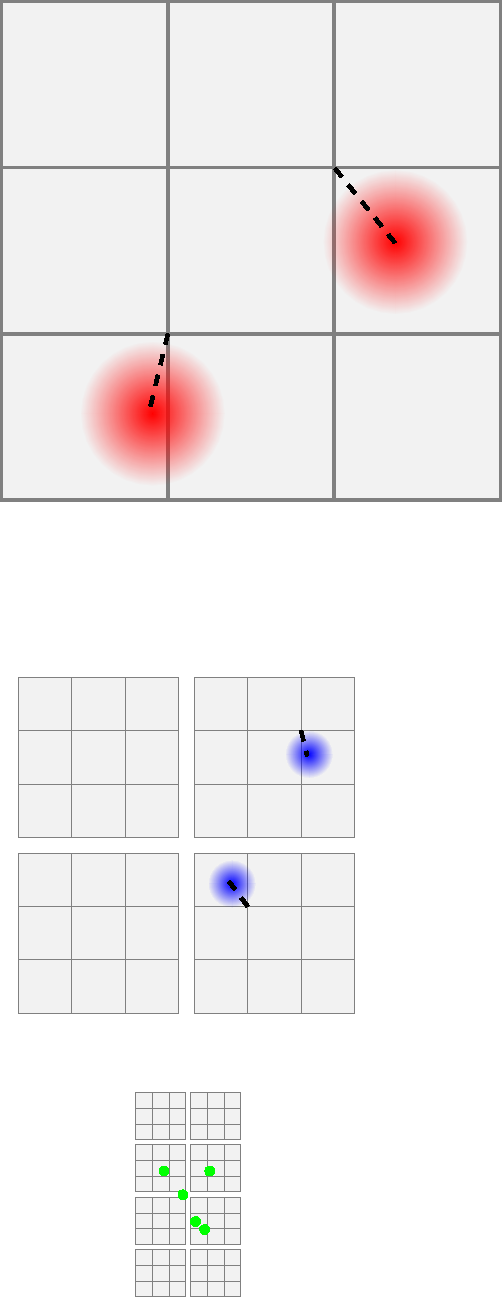
\includegraphics[width=0.25\textwidth]{61_pidt/dual-tree.pdf}
\end{center}

\noindent
A tree with three levels.
Particles with a large cut-off radius (red) are held on rather coarse levels.
Particles with very small cut-off are sorted (dropped) into the fine grid
levels.
Each particle is always associated to its closest vertex (dotted line).
It is the mesh which holds (owns) the vertices.
The toolset's predefined action set can automatically maintain/update these
associations after each grid sweep.
It also moves particles up and down the grid hierarchy if the particles' cut-off
radius changes or the grid changes.



\begin{definition}
  Our storage is vertex-oriented whereas most particle literature stores
  particles within cells.
  If we think of a dual multiscale mesh, i.e.~a mesh that is shifed by $h/2$
  alon each coordinate axis, then \Peano's approach also works with cells.
  Such shifted meshes are often called \emph{dual} meshes and I therefore speak
  of a \emph{dual tree}.
\end{definition}


\subsection{Dual tree traversal}

\Peano\ always runs through the mesh top-down, i.e.~it traverses the spacetree
in a depth-first fashion.


\section*{Links and further reading}

\begin{itemize}
  \item The ``official'' pidt paper is
{\tiny \begin{verbatim}
@article{WEINZIERL201642,
title = "Two particle-in-grid realisations on spacetrees",
journal = "Parallel Computing",
volume = "52",
pages = "42 - 64",
year = "2016",
issn = "0167-8191",
doi = "https://doi.org/10.1016/j.parco.2015.12.007",
url = "http://www.sciencedirect.com/science/article/pii/S0167819115001635",
author = "T. Weinzierl and B. Verleye and P. Henri and D. Roose",
keywords = "Particle-in-cell, Spacetree, Particle sorting, AMR, Lagrangian–Eulerian methods, Communication-avoiding"
}  \end{verbatim}}
  If you use the software, it would be great if you could cite this one.
\end{itemize}


